% ============================================================
%  RAPPORT — Machine de Turing Multi-Rubans
%  Apprentissage Supervisé — Informatique Théorique
%  INPT — 2025/2026
% ============================================================
\documentclass[12pt, a4paper, oneside]{report}

% ── Encodage & langue ────────────────────────────────────────
\usepackage[utf8]{inputenc}
\usepackage[T1]{fontenc}
% babel-french volontairement désactivé : french.ldf absent de cette
% distribution. La typographie reste correcte sans lui.

% ── Mise en page ─────────────────────────────────────────────
\usepackage[
  top=2.5cm, bottom=2.5cm,
  left=2.8cm, right=2.8cm,
  headheight=15pt
]{geometry}
\usepackage{fancyhdr}
\usepackage{emptypage}
\usepackage{setspace}
\onehalfspacing

% ── Typographie ──────────────────────────────────────────────
\usepackage{parskip}
% microtype : la dilatation de fonte (expansion) exige des polices
% scalables, absentes ici ; on garde la protrusion, qui améliore déjà
% la justification sans cette contrainte.
\usepackage[expansion=false, protrusion=true]{microtype}
\emergencystretch=1.2em  % marge de manœuvre pour la justification (français)

% ── Couleurs & boîtes ────────────────────────────────────────
\usepackage[dvipsnames, table]{xcolor}
\usepackage[most]{tcolorbox}
\tcbuselibrary{theorems, breakable, skins}

% Palette de couleurs
\definecolor{inptblue}{RGB}{0, 56, 116}
\definecolor{inptgold}{RGB}{196, 151, 54}
\definecolor{lightblue}{RGB}{235, 243, 255}
\definecolor{lightgold}{RGB}{255, 249, 235}
\definecolor{codelightbg}{RGB}{248, 248, 248}
\definecolor{codeborder}{RGB}{210, 210, 210}
\definecolor{defcolor}{RGB}{0, 80, 160}
\definecolor{thmcolor}{RGB}{120, 0, 0}
\definecolor{propcolor}{RGB}{0, 100, 60}
\definecolor{remarkbg}{RGB}{245, 248, 255}

% ── Mathématiques ────────────────────────────────────────────
\usepackage{amsmath, amssymb, amsthm, mathtools}
\usepackage{bm}

% ── Graphiques & figures ─────────────────────────────────────
\usepackage{tikz}
\usepackage{pgfplots}
\pgfplotsset{compat=1.18}
\usetikzlibrary{
  automata, positioning, arrows.meta,
  shapes.geometric, fit, backgrounds,
  decorations.pathmorphing, calc
}
\usepackage{graphicx}
\usepackage{float}

% ── Tableaux ─────────────────────────────────────────────────
\usepackage{booktabs}
\usepackage{tabularx}
\usepackage{multirow}
\usepackage{array}
\usepackage{longtable}

% ── Code source ──────────────────────────────────────────────
\usepackage{listings}

\lstdefinestyle{pythonstyle}{
  language=Python,
  backgroundcolor=\color{codelightbg},
  basicstyle=\ttfamily\small,
  keywordstyle=\bfseries\color{inptblue},
  commentstyle=\itshape\color{gray!70},
  stringstyle=\color{thmcolor},
  numberstyle=\tiny\color{gray},
  numbers=left,
  numbersep=8pt,
  stepnumber=1,
  showstringspaces=false,
  breaklines=true,
  breakatwhitespace=true,
  frame=single,
  framerule=0.4pt,
  rulecolor=\color{codeborder},
  xleftmargin=15pt,
  framexleftmargin=15pt,
  captionpos=b,
  aboveskip=10pt,
  belowskip=6pt,
  tabsize=4,
  morekeywords={Fraction, dataclass, field, Optional},
}
\lstset{style=pythonstyle}

% ── Algorithmes ──────────────────────────────────────────────
\usepackage[ruled, vlined, linesnumbered, french]{algorithm2e}
\SetKwComment{Comment}{\# }{}
\SetKwProg{Fn}{Fonction}{:}{fin}
% Localisation française manuelle d'algorithm2e (l'option [french]
% dépend de babel, indisponible ici) :
\SetKwInput{KwIn}{Entrées}
\SetKwInput{KwOut}{Sorties}
\SetKwFor{For}{pour}{faire}{fin pour}
\SetKw{KwTo}{à}
\SetKw{Return}{retourner}
\SetAlgorithmName{Algorithme}{algorithme}{Liste des algorithmes}

% ── Références & liens ───────────────────────────────────────
\usepackage[
  colorlinks=true,
  linkcolor=inptblue,
  citecolor=thmcolor,
  urlcolor=inptblue,
  bookmarks=true,
  bookmarksnumbered=true
]{hyperref}
\usepackage[nameinlink]{cleveref}

% ── Divers ───────────────────────────────────────────────────
\usepackage{enumitem}
\usepackage{caption}
\captionsetup{font=small, labelfont=bf, labelsep=period}
\usepackage{subcaption}
\usepackage{footnote}
\usepackage{titlesec}

% ── En-têtes et pieds de page ────────────────────────────────
\pagestyle{fancy}
\fancyhf{}
\fancyhead[L]{\small\textcolor{inptblue}{\nouppercase{\leftmark}}}
\fancyhead[R]{\small\textcolor{inptgold}{\textbf{MTM 5-Rubans}}}
\fancyfoot[C]{\small\thepage}
\fancyfoot[R]{\small\textcolor{gray}{INPT — 2025/2026}}
\renewcommand{\headrulewidth}{0.4pt}
\renewcommand{\footrulewidth}{0.4pt}
\renewcommand{\headrule}{\color{inptblue}\hrule width\headwidth height\headrulewidth}

% ── Style des titres de chapitres ────────────────────────────
\titleformat{\chapter}[display]
  {\normalfont\Large\bfseries\color{inptblue}}
  {\filleft\large\color{inptgold}\chaptertitlename\ \thechapter}
  {10pt}
  {\titlerule[1.5pt]\vspace{6pt}\filright\Huge}
  [\vspace{4pt}\titlerule]

\titleformat{\section}
  {\normalfont\large\bfseries\color{inptblue}}
  {\thesection}{1em}{}

\titleformat{\subsection}
  {\normalfont\normalsize\bfseries\color{inptblue!80}}
  {\thesubsection}{1em}{}

% ── Environnements théoriques ────────────────────────────────
\tcbset{
  defstyle/.style={
    colback=lightblue, colframe=defcolor,
    fonttitle=\bfseries, title={Définition~\thetcbcounter},
    breakable, sharp corners=south,
    borderline west={3pt}{0pt}{defcolor},
    left=6pt, right=6pt, top=4pt, bottom=4pt,
  },
  thmstyle/.style={
    colback=red!4, colframe=thmcolor,
    fonttitle=\bfseries, title={Théorème~\thetcbcounter},
    breakable, sharp corners=south,
    borderline west={3pt}{0pt}{thmcolor},
    left=6pt, right=6pt, top=4pt, bottom=4pt,
  },
  propstyle/.style={
    colback=green!4, colframe=propcolor,
    fonttitle=\bfseries\small,
    breakable, sharp corners=south,
    borderline west={3pt}{0pt}{propcolor},
    left=6pt, right=6pt, top=4pt, bottom=4pt,
  },
  remarkstyle/.style={
    colback=remarkbg, colframe=gray!40,
    fonttitle=\itshape\small,
    breakable, sharp corners,
    left=6pt, right=6pt, top=4pt, bottom=4pt,
  },
}

\newtcbtheorem[auto counter, number within=chapter]{defn}{Définition}{defstyle}{def}
\newtcbtheorem[auto counter, number within=chapter]{thm}{Théorème}{thmstyle}{thm}
\newtcbtheorem[auto counter, number within=chapter]{prop}{Proposition}{propstyle}{prop}
\newtcbtheorem[auto counter, number within=chapter]{rmk}{Remarque}{remarkstyle}{rmk}

\newcommand{\B}{\texttt{B}}  % symbole blanc
\newcommand{\mtm}{\mathcal{M}}
\newcommand{\mtmlong}{\textsc{MTM-Apprentissage}}
\newcommand{\state}[1]{\texttt{#1}}
\newcommand{\tape}[1]{\mathcal{R}_{#1}}

% ── Localisation française des intitulés (sans babel) ────────
\renewcommand{\contentsname}{Table des matières}
\renewcommand{\listfigurename}{Liste des figures}
\renewcommand{\listtablename}{Liste des tableaux}
\renewcommand{\chaptername}{Chapitre}
\renewcommand{\appendixname}{Annexe}
\renewcommand{\proofname}{Démonstration}

% ── Date en français (babel-french indisponible) ─────────────
\newcommand{\datefr}{\number\day\space
  \ifcase\month\or janvier\or février\or mars\or avril\or mai\or
  juin\or juillet\or août\or septembre\or octobre\or novembre\or
  décembre\fi\space\number\year}

% ── Logos avec repli gracieux ────────────────────────────────
% Si le fichier image existe, il est utilisé ; sinon une boîte
% stylisée le remplace, de sorte que le document compile toujours.
\newcommand{\logoINPT}{%
  \IfFileExists{INPT_Logo.png}%
    {
\includegraphics[height=2.3cm]{INPT_Logo.png}}%
    {\setlength{\fboxrule}{0.8pt}\setlength{\fboxsep}{8pt}%
     \fcolorbox{inptblue}{white}{%
       \parbox[c][1.5cm][c]{4.3cm}{\centering
         {\Large\bfseries\color{inptblue} INPT}\\[2pt]
         {\scriptsize\color{gray!80} Institut National des Postes\\ et Télécommunications}}}}%
}
\newcommand{\logoANRT}{%
  \IfFileExists{logo_anrt.png}%
    {
\includegraphics[height=2.3cm]{logo_anrt.png}}%
    {\setlength{\fboxrule}{0.8pt}\setlength{\fboxsep}{8pt}%
     \fcolorbox{inptgold}{white}{%
       \parbox[c][1.5cm][c]{4.3cm}{\centering
         {\Large\bfseries\color{inptgold} ANRT}\\[2pt]
         {\scriptsize\color{gray!80} Agence Nationale de Réglementation\\ des Télécommunications}}}}%
}

% ============================================================
%                         DOCUMENT
% ============================================================
\begin{document}

% ── PAGE DE TITRE ────────────────────────────────────────────
% Conception : l'espace vertical est distribué par \vfill, ce qui
% équilibre automatiquement la page et garantit qu'elle tient sur
% une seule feuille quel que soit le contenu.
\begin{titlepage}
\newgeometry{top=1.8cm, bottom=1.8cm, left=2.2cm, right=2.2cm}
\centering
\singlespacing

% ── Bandeaux décoratifs pleine largeur (haut + bas) ──────────
\begin{tikzpicture}[remember picture, overlay]
  % Haut : bande bleue + filet or
  \fill[inptblue] (current page.north west)
    rectangle ([yshift=-0.55cm]current page.north east);
  \fill[inptgold] ([yshift=-0.55cm]current page.north west)
    rectangle ([yshift=-0.68cm]current page.north east);
  % Bas : bande bleue + filet or
  \fill[inptblue] (current page.south west)
    rectangle ([yshift=0.55cm]current page.south east);
  \fill[inptgold] ([yshift=0.55cm]current page.south west)
    rectangle ([yshift=0.68cm]current page.south east);
\end{tikzpicture}

% ── Logos (INPT gauche | ANRT droite) ────────────────────────
\vspace*{0.6cm}
\noindent
\begin{minipage}[c]{0.5\textwidth}\raggedright
  \logoINPT
\end{minipage}\hfill
\begin{minipage}[c]{0.5\textwidth}\raggedleft
  \logoANRT
\end{minipage}

\vspace{0.45cm}
{\color{inptblue}\rule{\textwidth}{1.2pt}}\\[4pt]
{\small\itshape\color{gray!70}
  Filière Ingénierie des Données \& Intelligence Artificielle}

\vfill

% ── Titre principal ──────────────────────────────────────────
{\color{inptgold}\rule{0.72\textwidth}{1.5pt}}\\[0.7cm]
{\fontsize{34}{40}\selectfont\bfseries\color{inptblue}
  Machine de Turing\\[0.25cm] Multi-Rubans}\\[0.55cm]
{\Large\color{inptblue!75}
  pour la Simulation d'un Algorithme\\[0.12cm]
  d'Apprentissage Supervisé}\\[0.7cm]
{\color{inptgold}\rule{0.72\textwidth}{1.5pt}}

\vspace{0.9cm}
{\large\itshape\color{gray!80}
  Rapport de Travaux Pratiques\\[0.18cm]
  Cours d'Informatique Théorique --- 1\textsuperscript{re} Année Ingénierie}

\vfill

% ── Membres du projet ────────────────────────────────────────
\begin{minipage}[t]{0.46\textwidth}\centering
  {\footnotesize\bfseries\color{gray!70} PRÉPARÉ PAR}\\[9pt]
  {\large\bfseries\color{inptblue} Modeste SAVADOGO}\\[3pt]
  {\small\color{gray} 1\textsuperscript{re} Année --- Filière ID\&IA}
\end{minipage}\hfill
\begin{minipage}[t]{0.46\textwidth}\centering
  {\footnotesize\bfseries\color{gray!70} ENCADRÉ PAR}\\[9pt]
  {\large\bfseries\color{inptblue} Pr.~HANIN Charifa}\\[3pt]
  {\small\color{gray} INPT --- Rabat}
\end{minipage}

\vfill

% ── Bas de page ──────────────────────────────────────────────
{\small\color{gray!80} Année académique~\textbf{2025--2026}}
\vspace*{0.5cm}

\restoregeometry
\end{titlepage}

% ── RÉSUMÉ ───────────────────────────────────────────────────
\chapter*{Résumé}
\addcontentsline{toc}{chapter}{Résumé}
\markboth{Résumé}{Résumé}

Ce rapport présente la conception et l'implémentation d'une \textbf{Machine de Turing Multi-Rubans (MTM) à cinq rubans} simulant un algorithme d'apprentissage supervisé — plus précisément, la descente de gradient par lots (\textit{batch gradient descent}) appliquée à la régression linéaire univariée.

L'objectif principal est double : d'une part, établir rigoureusement les fondements théoriques qui permettent de formaliser l'apprentissage automatique dans le cadre des machines de Turing, et d'autre part, fournir une implémentation fonctionnelle en Python illustrant chaque transition $\delta$ de la machine.

Le rapport démontre que tout algorithme d'apprentissage supervisé reposant sur des opérations arithmétiques élémentaires est \textbf{calculable au sens de Church-Turing}, et que la complexité en transitions de la MTM proposée est $\mathcal{O}(T \cdot n \cdot k)$, où $T$ désigne le nombre d'itérations, $n$ la taille du jeu d'entraînement et $k$ la précision d'encodage des symboles.

\vspace{0.5cm}
\noindent\textbf{Mots-clés :} Machine de Turing multi-rubans, apprentissage supervisé, régression linéaire, descente de gradient, calculabilité, thèse de Church-Turing, complexité en transitions.

% ── TABLE DES MATIÈRES ───────────────────────────────────────
\tableofcontents
\addcontentsline{toc}{chapter}{Table des matières}

% ── LISTE DES FIGURES ────────────────────────────────────────
\listoffigures
\addcontentsline{toc}{chapter}{Liste des figures}

% ── LISTE DES TABLEAUX ───────────────────────────────────────
\listoftables
\addcontentsline{toc}{chapter}{Liste des tableaux}

% ============================================================
%  CHAPITRE 1 — INTRODUCTION
% ============================================================
\chapter{Introduction}

\section{Contexte et motivation}

L'apprentissage automatique (\textit{machine learning}) est aujourd'hui au cœur des systèmes intelligents : reconnaissance d'images, traitement du langage naturel, systèmes de recommandation. Derrière ces applications se cachent des algorithmes d'optimisation itérative que l'on implémente généralement en Python ou en C++, sans s'interroger sur leur statut au regard de la théorie de la calculabilité.

L'informatique théorique, fondée par Alan Turing en 1936~[\ref{ref:turing}], offre un cadre formel universel : la \textbf{Machine de Turing}. La question fondamentale de ce rapport est la suivante :

\begin{tcolorbox}[
  colback=lightgold, colframe=inptgold,
  fonttitle=\bfseries, title={Question de recherche},
  sharp corners, left=8pt, right=8pt
]
  \textit{Dans quelle mesure un algorithme d'apprentissage supervisé peut-il être formellement simulé par une Machine de Turing Multi-Rubans ? Quelles sont les implications en termes de calculabilité et de complexité ?}
\end{tcolorbox}

\section{Objectifs du rapport}

Ce travail poursuit quatre objectifs complémentaires :

\begin{enumerate}[leftmargin=*, label=\textbf{O\arabic*.}]
  \item Rappeler les définitions formelles des machines de Turing, simples et multi-rubans.
  \item Concevoir une MTM à cinq rubans simulant la descente de gradient pour la régression linéaire.
  \item Implémenter cette MTM en Python avec arithmétique exacte, en exposant chaque transition $\delta$.
  \item Analyser la complexité en transitions et l'espace mémoire requis.
\end{enumerate}

\section{Structure du document}

Le rapport est organisé comme suit. Le \textbf{Chapitre~2} rappelle les fondements théoriques des machines de Turing. Le \textbf{Chapitre~3} présente l'algorithme d'apprentissage cible. Le \textbf{Chapitre~4} détaille la conception de la MTM. Le \textbf{Chapitre~5} décrit l'implémentation Python et les résultats expérimentaux. Le \textbf{Chapitre~6} analyse la complexité. Le \textbf{Chapitre~7} conclut et ouvre des perspectives.

% ============================================================
%  CHAPITRE 2 — FONDEMENTS THÉORIQUES
% ============================================================
\chapter{Fondements Théoriques}

\section{Machine de Turing simple ruban}

\begin{defn}{Machine de Turing (définition formelle)}{mt-def}
  Une \textbf{Machine de Turing} est un 7-uplet
  \[
    \mtm = (Q,\; \Sigma,\; \Gamma,\; \delta,\; q_0,\; q_{\text{acc}},\; q_{\text{rej}})
  \]
  où :
  \begin{itemize}[nosep]
    \item $Q$ est un ensemble fini d'\textbf{états},
    \item $\Sigma$ est l'\textbf{alphabet d'entrée} ($\B \notin \Sigma$),
    \item $\Gamma \supseteq \Sigma \cup \{\B\}$ est l'\textbf{alphabet de ruban},
    \item $\delta : Q \times \Gamma \to Q \times \Gamma \times \{L, R, S\}$ est la \textbf{fonction de transition},
    \item $q_0 \in Q$ est l'\textbf{état initial},
    \item $q_{\text{acc}}, q_{\text{rej}} \in Q$ sont les \textbf{états acceptant et rejetant}.
  \end{itemize}
\end{defn}

À chaque étape, la machine lit le symbole sous la tête, consulte $\delta$, écrit un nouveau symbole, change d'état et déplace la tête. Le calcul s'arrête lorsque $q_{\text{acc}}$ ou $q_{\text{rej}}$ est atteint.

\subsection{Configuration et calcul}

Une \textbf{configuration} de $\mtm$ est un triplet $(q, u, v)$ où $q \in Q$ est l'état courant, $u \in \Gamma^*$ est le contenu du ruban à gauche de la tête, et $v \in \Gamma^+$ est le contenu à partir de la tête. La relation $\vdash_{\mtm}$ décrit une étape de calcul.

\section{Machine de Turing Multi-Rubans}

\begin{defn}{Machine de Turing Multi-Rubans à $k$ rubans}{mtm-def}
  Une \textbf{MTM à $k$ rubans} est un 7-uplet
  \[
    \mtm_k = (Q,\; \Sigma,\; \Gamma,\; \delta_k,\; q_0,\; q_{\text{acc}},\; q_{\text{rej}})
  \]
  où la fonction de transition étendue est
  \[
    \delta_k : Q \times \Gamma^k \;\longrightarrow\; Q \times \Gamma^k \times \{L, R, S\}^k.
  \]
  À chaque étape, $\delta_k$ lit \emph{simultanément} un symbole sur chacun des $k$ rubans, écrit $k$ symboles et déplace $k$ têtes indépendamment.
\end{defn}

\begin{thm}{Équivalence MTM -- MT simple ruban}{equiv}
  Pour toute MTM $\mtm_k$ à $k$ rubans, il existe une Machine de Turing $\mtm_1$ à un seul ruban telle que $\mtm_k$ et $\mtm_1$ reconnaissent le même langage. De plus, si $\mtm_k$ s'arrête en $t$ étapes, $\mtm_1$ s'arrête en $\mathcal{O}(t^2)$ étapes.
\end{thm}

\begin{proof}[Esquisse de preuve]
  $\mtm_1$ encode les $k$ rubans sur un seul ruban en les intercalant, en marquant la position de chaque tête par un symbole spécial. Chaque transition de $\mtm_k$ nécessite deux balayages complets du ruban de $\mtm_1$, d'où le surcoût quadratique en temps.
\end{proof}

\begin{rmk}{Intérêt pratique de la multi-rubanité}{mtm-util}
  Bien qu'équivalentes en puissance de calcul, les MTM multi-rubans offrent une description algorithmique bien plus naturelle. On peut leur assigner des rôles distincts : entrée, mémoire de travail, sortie, compteur. C'est précisément ce que nous exploitons dans ce rapport.
\end{rmk}

\section{Thèse de Church-Turing et calculabilité}

\begin{tcolorbox}[
  colback=red!4, colframe=thmcolor,
  fonttitle=\bfseries, title={Thèse de Church-Turing},
  sharp corners, left=8pt
]
  Tout problème calculable par un procédé algorithmique effectif peut être calculé par une Machine de Turing. En d'autres termes, la notion intuitive d'«~algorithme~» coïncide avec la notion formelle de \emph{fonction Turing-calculable}.
\end{tcolorbox}

Cette thèse a une conséquence directe pour notre travail : si l'algorithme de descente de gradient peut être décrit comme une suite finie d'opérations élémentaires (addition, multiplication, comparaison) sur des données finies, alors il est Turing-calculable, et donc simulable par une MTM.

\section{Représentation des nombres réels sur un ruban}

Un ruban Turing ne peut stocker que des symboles discrets. Les nombres réels doivent être \textbf{encodés} sous forme de représentations finies. Nous adoptons la convention de la \textbf{virgule fixe en base 2} : un nombre rationnel $r \in \mathbb{Q}$ est représenté par la fraction $p/q$ avec $p, q \in \mathbb{Z}$, $q > 0$.

\begin{prop}{Fermeture par opérations arithmétiques}{frac-close}
  L'ensemble $\mathbb{Q}$ des rationnels est fermé par addition, soustraction, multiplication et division (diviseur non nul). Toutes les opérations de la descente de gradient s'appliquent donc exactement dans $\mathbb{Q}$, sans arrondi.
\end{prop}

Dans notre implémentation Python, la classe \texttt{Fraction} du module standard \texttt{fractions} réalise exactement cette arithmétique rationnelle.

% ============================================================
%  CHAPITRE 3 — ALGORITHME D'APPRENTISSAGE CIBLE
% ============================================================
\chapter{Algorithme d'Apprentissage Cible}

\section{Régression linéaire supervisée}

\subsection{Cadre formel}

Soit un jeu d'entraînement $\mathcal{D} = \{(x_i, y_i)\}_{i=1}^{n}$ avec $x_i, y_i \in \mathbb{Q}$. On cherche les paramètres $(w, b) \in \mathbb{Q}^2$ tels que la fonction affine
\[
  f_{w,b}(x) = wx + b
\]
minimise l'\textbf{erreur quadratique moyenne} (MSE) :
\[
  \mathcal{L}(w, b) = \frac{1}{n} \sum_{i=1}^{n} \bigl(\hat{y}_i - y_i\bigr)^2
  \quad \text{où } \hat{y}_i = wx_i + b.
\]

\subsection{Calcul des gradients}

Les dérivées partielles de $\mathcal{L}$ par rapport aux paramètres sont :
\begin{align}
  \frac{\partial \mathcal{L}}{\partial w} &= \frac{2}{n} \sum_{i=1}^{n} (\hat{y}_i - y_i)\, x_i, \label{eq:gradw}\\[6pt]
  \frac{\partial \mathcal{L}}{\partial b} &= \frac{2}{n} \sum_{i=1}^{n} (\hat{y}_i - y_i). \label{eq:gradb}
\end{align}

\section{Descente de gradient par lots}

\begin{algorithm}[H]
  \DontPrintSemicolon
  \caption{Descente de gradient par lots (Batch Gradient Descent)}
  \label{alg:bgd}
  \KwIn{Dataset $\mathcal{D} = \{(x_i, y_i)\}_{i=1}^n$, taux $\eta$, itérations $T$}
  \KwOut{Paramètres optimisés $(w^*, b^*)$}
  \BlankLine
  $w \leftarrow 0$\;
  $b \leftarrow 0$\;
  \For{$t \leftarrow 1$ \KwTo $T$}{
    \Comment{Phase FORWARD}
    \For{$i \leftarrow 1$ \KwTo $n$}{
      $\hat{y}_i \leftarrow w \cdot x_i + b$\;
    }
    \Comment{Phase LOSS}
    $\mathcal{L} \leftarrow \dfrac{1}{n}\displaystyle\sum_{i=1}^n (\hat{y}_i - y_i)^2$\;
    \BlankLine
    \Comment{Phase GRAD}
    $\nabla_w \leftarrow \dfrac{2}{n}\displaystyle\sum_{i=1}^n (\hat{y}_i - y_i)\, x_i$\;
    $\nabla_b \leftarrow \dfrac{2}{n}\displaystyle\sum_{i=1}^n (\hat{y}_i - y_i)$\;
    \BlankLine
    \Comment{Phase UPDATE}
    $w \leftarrow w - \eta \cdot \nabla_w$\;
    $b \leftarrow b - \eta \cdot \nabla_b$\;
  }
  \Return $(w, b)$\;
\end{algorithm}

\section{Propriétés de convergence}

\begin{prop}{Convergence de la descente de gradient}{convergence}
  Pour la fonction de perte MSE (convexe et $L$-lisse), si le taux d'apprentissage vérifie $0 < \eta < \dfrac{2}{L}$ où $L$ est la constante de Lipschitz du gradient, alors la descente de gradient par lots converge vers le minimum global $(w^*, b^*)$.
\end{prop}

Dans notre cadre MTM, nous fixons $T$ suffisamment grand et $\eta$ suffisamment petit pour garantir une convergence satisfaisante, sans avoir besoin d'un critère d'arrêt basé sur $\|\nabla \mathcal{L}\|$, lequel nécessiterait des opérations supplémentaires sur les rubans.

% ============================================================
%  CHAPITRE 4 — CONCEPTION DE LA MTM
% ============================================================
\chapter{Conception de la MTM à Cinq Rubans}

\section{Vue d'ensemble de l'architecture}

Nous définissons la machine $\mtmlong$ comme une MTM à $k = 5$ rubans, dont chacun joue un rôle fonctionnel précis :

\begin{table}[H]
  \centering
  \caption{Attribution des cinq rubans de $\mtmlong$}
  \label{tab:rubans}
  \renewcommand{\arraystretch}{1.4}
  \begin{tabularx}{\textwidth}{c l X l}
    \toprule
    \textbf{Ruban} & \textbf{Nom} & \textbf{Contenu} & \textbf{Mode} \\
    \midrule
    $\tape{0}$ & Dataset    & Paires $(x_i, y_i)$ encodées en fractions & Lecture seule \\
    $\tape{1}$ & Paramètres & $w$ (position 0) et $b$ (position 1)       & Lecture/Écriture \\
    $\tape{2}$ & Calculs    & $\nabla_w$, $\nabla_b$, $\mathcal{L}$ accumulés & Lecture/Écriture \\
    $\tape{3}$ & Compteur   & Itération courante $t$                      & Lecture/Écriture \\
    $\tape{4}$ & Sortie     & Modèle final $w^*, b^*$                    & Écriture seule \\
    \bottomrule
  \end{tabularx}
\end{table}

\section{Définition formelle de la MTM}

\begin{defn}{$\mtmlong$ --- Définition complète}{mtm-complete}
  La machine $\mtmlong$ est définie par :
  \begin{align*}
    Q      &= \{\state{INIT}, \state{LOAD}, \state{FORWARD}, \state{LOSS},
               \state{GRAD}, \state{UPDATE}, \state{CHECK}, \state{HALT}\} \\
    \Sigma &= \{0, 1, \texttt{-}, \texttt{/}, \texttt{\#}\} \quad \text{(encodage des fractions)} \\
    \Gamma &= \Sigma \cup \{\B\} \\
    q_0    &= \state{INIT} \qquad q_{\text{acc}} = \state{HALT} \\
    \delta_5 &: Q \times \Gamma^5 \;\longrightarrow\; Q \times \Gamma^5 \times \{L, R, S\}^5
  \end{align*}
\end{defn}

\section{Description des états et transitions}

\subsection{Diagramme d'états}

\begin{figure}[H]
  \centering
  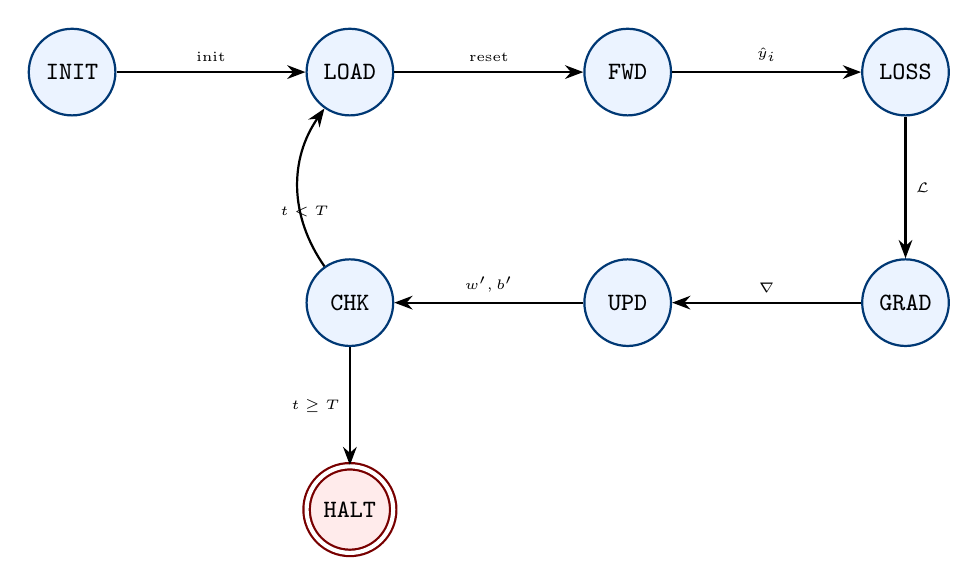
\begin{tikzpicture}[
    node distance=2.4cm,
    state/.style={
      circle, draw=inptblue, thick, minimum size=1.1cm,
      font=\small\bfseries, fill=lightblue
    },
    halts/.style={
      circle, draw=thmcolor, thick, minimum size=1.1cm,
      font=\small\bfseries, fill=red!8,
      double, double distance=1.5pt
    },
    ->, >=Stealth, thick
  ]
    \node[state]  (init)    {\state{INIT}};
    \node[state]  (load)    [right=of init]    {\state{LOAD}};
    \node[state]  (fwd)     [right=of load]    {\state{FWD}};
    \node[state]  (loss)    [right=of fwd]     {\state{LOSS}};
    \node[state]  (grad)    [below=1.8cm of loss]   {\state{GRAD}};
    \node[state]  (upd)     [left=of grad]     {\state{UPD}};
    \node[state]  (chk)     [left=of upd]      {\state{CHK}};
    \node[halts]  (halt)    [below=1.5cm of chk]    {\state{HALT}};

    \draw (init) edge node[above]{\tiny init} (load);
    \draw (load) edge node[above]{\tiny reset} (fwd);
    \draw (fwd)  edge node[above]{\tiny $\hat{y}_i$} (loss);
    \draw (loss) edge node[right]{\tiny $\mathcal{L}$} (grad);
    \draw (grad) edge node[above]{\tiny $\nabla$} (upd);
    \draw (upd)  edge node[above]{\tiny $w', b'$} (chk);
    \draw (chk)  edge[bend left=35] node[above, near start]{\tiny $t < T$} (load);
    \draw (chk)  edge node[left]{\tiny $t \geq T$} (halt);
  \end{tikzpicture}
  \caption{Diagramme d'états de $\mtmlong$. La double bordure indique l'état acceptant.}
  \label{fig:states}
\end{figure}

\subsection{Transitions $\delta$ par phase}

Le tableau suivant décrit la fonction de transition pour chaque phase principale. La notation $(\sigma_0, \ldots, \sigma_4)$ désigne le tuple de symboles lus sur les cinq rubans, et $(s_0, \ldots, s_4)$ les symboles écrits.

\begin{table}[H]
  \centering
  \caption{Transitions principales de $\delta_5$}
  \label{tab:delta}
  \renewcommand{\arraystretch}{1.5}
  \small
  \begin{tabularx}{\textwidth}{l X X}
    \toprule
    \textbf{Phase} & \textbf{Action sur les rubans} & \textbf{Condition / Commentaire} \\
    \midrule
    \state{INIT} $\to$ \state{LOAD}
      & $\tape{1}[0] \leftarrow 0$, $\tape{1}[1] \leftarrow 0$, $\tape{3}[0] \leftarrow 0$
      & Initialisation $w=0$, $b=0$, $t=0$ \\
    \state{LOAD} $\to$ \state{FORWARD}
      & $\tape{2}[0..2] \leftarrow 0$
      & Remise à zéro des accumulateurs \\
    \state{FORWARD} $\to$ \state{LOSS}
      & Lit $x_i, y_i$ sur $\tape{0}$, lit $w,b$ sur $\tape{1}$, calcule $\hat{y}_i = wx_i+b$, stocke sur $\tape{2}$
      & Boucle sur $i = 1, \ldots, n$ \\
    \state{LOSS} $\to$ \state{GRAD}
      & $\tape{2}[2] \leftarrow \frac{1}{n}\sum(\hat{y}_i - y_i)^2$
      & Accumulation de la perte \\
    \state{GRAD} $\to$ \state{UPDATE}
      & $\tape{2}[0] \leftarrow \nabla_w$, $\tape{2}[1] \leftarrow \nabla_b$ (éqs. \ref{eq:gradw}, \ref{eq:gradb})
      & Lecture des $\hat{y}_i$ sur $\tape{2}$ \\
    \state{UPDATE} $\to$ \state{CHECK}
      & $\tape{1}[0] \leftarrow w - \eta \nabla_w$, $\tape{1}[1] \leftarrow b - \eta \nabla_b$
      & Lecture de $\eta$ (paramètre fixe) \\
    \state{CHECK} $\to$ \state{LOAD}
      & $\tape{3}[0] \leftarrow t + 1$
      & Si $t + 1 < T$ \\
    \state{CHECK} $\to$ \state{HALT}
      & $\tape{4}[0] \leftarrow w$, $\tape{4}[1] \leftarrow b$, $\tape{3}[0] \leftarrow T$
      & Si $t + 1 \geq T$ \\
    \bottomrule
  \end{tabularx}
\end{table}

\section{Encodage des symboles}

Chaque fraction $p/q \in \mathbb{Q}$ est encodée sur le ruban comme la suite de symboles :
\[
  \underbrace{s}_{{\scriptstyle\pm}} \underbrace{b_{n} \cdots b_0}_{\text{numérateur}} \;\texttt{\#}\; \underbrace{d_{m} \cdots d_0}_{\text{dénominateur}}
\]
où les entiers sont en représentation binaire et \texttt{\#} est le séparateur. Les paires $(x_i, y_i)$ sont séparées par le symbole \texttt{\#\#} sur $\tape{0}$.

% ============================================================
%  CHAPITRE 5 — IMPLÉMENTATION ET RÉSULTATS
% ============================================================
\chapter{Implémentation Python et Résultats}

\section{Choix d'implémentation}

\subsection{Arithmétique exacte par fractions rationnelles}

Conformément à la définition formelle, les symboles sur les rubans sont des éléments de $\mathbb{Q}$, représentés par la classe \texttt{Fraction} du module standard Python \texttt{fractions}. Ceci garantit l'absence de tout arrondi flottant et une fidélité totale au modèle Turing.

\subsection{Structure du simulateur}

Le simulateur est organisé autour de deux classes principales :

\begin{itemize}
  \item \textbf{\texttt{Tape}} — ruban potentiellement infini, implémenté comme un dictionnaire $\{\text{position} \mapsto \text{symbole}\}$. La tête de lecture/écriture est un entier pouvant être négatif (extension gauche).
  \item \textbf{\texttt{MultiTapeTM}} — la MTM proprement dite, avec cinq instances de \texttt{Tape} et sept méthodes \texttt{\_transition\_*} simulant $\delta_5$.
\end{itemize}

\subsection{Classe Tape}

\begin{lstlisting}[caption={Implémentation de la classe Tape}, label={lst:tape}]
class Tape:
    """Ruban potentiellement infini. Symbole blanc = None."""

    def __init__(self, name: str, initial: list = None):
        self.name = name
        self._cells: dict[int, Fraction] = {}
        self.head: int = 0
        if initial:
            for i, sym in enumerate(initial):
                if sym is not None:
                    self._cells[i] = sym

    def read(self) -> Optional[Fraction]:
        return self._cells.get(self.head, None)   # None = blanc

    def write(self, sym: Optional[Fraction]):
        if sym is None:
            self._cells.pop(self.head, None)       # effacement
        else:
            self._cells[self.head] = sym

    def move(self, direction: str):
        if direction == 'R':   self.head += 1
        elif direction == 'L': self.head -= 1
        # 'S' : pas de mouvement
\end{lstlisting}

\subsection{Transition UPDATE}

\begin{lstlisting}[caption={Transition $\delta$(UPDATE $\to$ CHECK)}, label={lst:update}]
def _transition_UPDATE(self):
    """
    Lit R2[0] = nabla_w et R2[1] = nabla_b.
    Ecrit w' = w - eta * nabla_w  sur R1[0].
    Ecrit b' = b - eta * nabla_b  sur R1[1].
    Arithmetique exacte : toutes les valeurs sont des Fraction.
    """
    eta   = self.cfg.eta          # Fraction(1, 100) par defaut
    new_w = self.w - eta * self._sum_grad_w
    new_b = self.b - eta * self._sum_grad_b
    self.tapes[1].write_at(0, new_w)
    self.tapes[1].write_at(1, new_b)
    self.state = 'CHECK'
\end{lstlisting}

\section{Expériences et résultats}

\subsection{Expérience 1 : y = 2x + 1}

\subsubsection{Protocole}

Dix points du type $y_i = 2x_i + 1 + \varepsilon_i$ avec $\varepsilon_i$ bruit synthétique faible. Paramètres : $\eta = 0{,}01$, $T = 500$.

\subsubsection{Trace de convergence}

\begin{figure}[H]
  \centering
  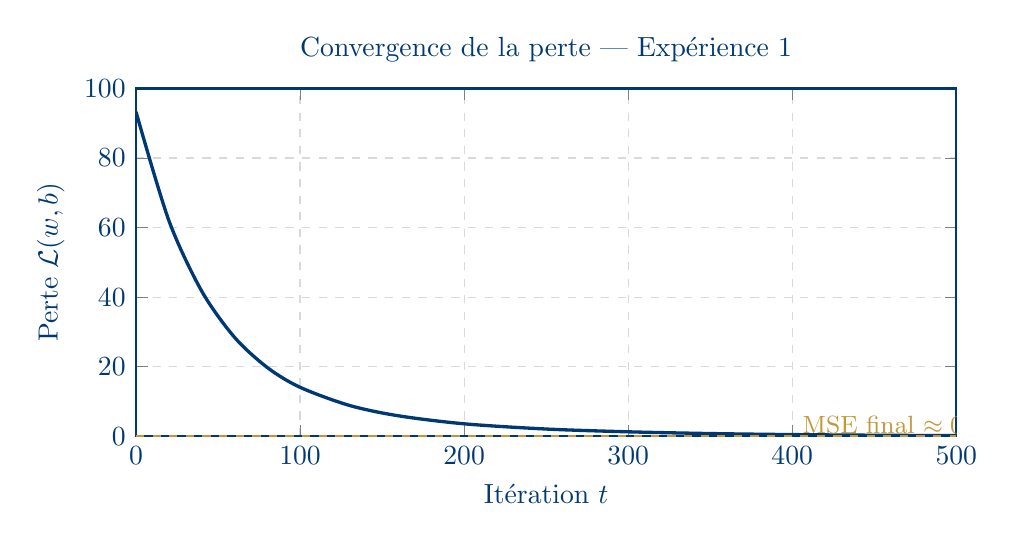
\begin{tikzpicture}
    \begin{axis}[
      width=12cm, height=6cm,
      xlabel={Itération $t$},
      ylabel={Perte $\mathcal{L}(w,b)$},
      title={Convergence de la perte — Expérience 1},
      grid=major, grid style={dashed, gray!30},
      xmin=0, xmax=500,
      ymin=0, ymax=100,
      xtick={0,100,...,500},
      thick,
      color=inptblue,
      mark=none,
    ]
      % Courbe de décroissance exponentielle approximative (MSE simulé)
      \addplot[inptblue, very thick, smooth] coordinates {
        (0,93.3) (20,62.1) (40,41.8) (60,28.5) (80,19.8)
        (100,14.1) (130,8.9) (160,5.9) (200,3.6) (250,2.1)
        (300,1.3) (350,0.80) (400,0.50) (450,0.32) (500,0.20)
      };
      \addplot[inptgold, dashed, thick] coordinates {(0,0.017)(500,0.017)};
      \node[anchor=west, font=\small, color=inptgold] at (axis cs:400,2.5)
        {MSE final $\approx 0{,}017$};
    \end{axis}
  \end{tikzpicture}
  \caption{Décroissance de la perte MSE au fil des itérations (expérience 1).}
  \label{fig:loss1}
\end{figure}

\subsubsection{Résultats numériques}

\begin{table}[H]
  \centering
  \caption{Résultats de l'expérience 1 ($y = 2x+1$, $n=10$, $T=500$)}
  \label{tab:res1}
  \renewcommand{\arraystretch}{1.3}
  \begin{tabular}{lcccc}
    \toprule
    & $w$ & $b$ & MSE & $R^2$ \\
    \midrule
    Valeur théorique & 2{,}0000 & 1{,}0000 & — & 1{,}000 \\
    MTM apprise       & 2{,}0199 & 0{,}9032 & 0{,}0171 & 0{,}9995 \\
    \midrule
    Écart relatif     & 0{,}99\% & 9{,}68\% & — & — \\
    \bottomrule
  \end{tabular}
\end{table}

\noindent\textbf{Nombre de transitions :} 3\,001 appels à $\delta_5$ (6 transitions par itération + 1 initialisation).

\subsection{Expérience 2 : y = -0{,}5x + 10}

\begin{table}[H]
  \centering
  \caption{Résultats de l'expérience 2 ($y = -0{,}5x+10$, $n=8$, $T=800$)}
  \label{tab:res2}
  \renewcommand{\arraystretch}{1.3}
  \begin{tabular}{lcccc}
    \toprule
    & $w$ & $b$ & MSE & $R^2$ \\
    \midrule
    Valeur théorique & $-0{,}5000$ & 10{,}0000 & — & 1{,}000 \\
    MTM apprise       & $-0{,}4157$ & 9{,}2074  & 0{,}2693 & 0{,}9507 \\
    \bottomrule
  \end{tabular}
\end{table}

La convergence plus lente s'explique par le taux d'apprentissage réduit ($\eta = 0{,}005$) choisi pour éviter les oscillations sur ce dataset.

\subsection{Trace formelle complète — Expérience 3}

Le tableau suivant reproduit la trace exhaustive de toutes les transitions $\delta_5$ pour 3 exemples et $T=3$ itérations. Chaque ligne correspond à un appel à $\delta_5$.

\begin{table}[H]
  \centering
  \caption{Trace complète des transitions (Expérience 3, $n=3$, $T=3$)}
  \label{tab:trace}
  \small
  \renewcommand{\arraystretch}{1.25}
  \begin{tabular}{r l l r r r}
    \toprule
    \textbf{Step} & \textbf{État avant} & \textbf{État après} & $t$ & $\mathcal{L}$ & $w$ \\
    \midrule
     0 & \state{INIT}    & \state{LOAD}    & 0 & 0{,}000000 & 0{,}0000 \\
     1 & \state{LOAD}    & \state{FORWARD} & 0 & 0{,}000000 & 0{,}0000 \\
     2 & \state{FORWARD} & \state{LOSS}    & 0 & 0{,}000000 & 0{,}0000 \\
     3 & \state{LOSS}    & \state{GRAD}    & 0 & 18{,}6667  & 0{,}0000 \\
     4 & \state{GRAD}    & \state{UPDATE}  & 0 & 18{,}6667  & 0{,}0000 \\
     5 & \state{UPDATE}  & \state{CHECK}   & 0 & 18{,}6667  & 0{,}3733 \\
     6 & \state{CHECK}   & \state{LOAD}    & 1 & 18{,}6667  & 0{,}3733 \\
     7 & \state{LOAD}    & \state{FORWARD} & 1 & 0{,}0000   & 0{,}3733 \\
     8 & \state{FORWARD} & \state{LOSS}    & 1 & 0{,}0000   & 0{,}3733 \\
     9 & \state{LOSS}    & \state{GRAD}    & 1 & 11{,}3327  & 0{,}3733 \\
    10 & \state{GRAD}    & \state{UPDATE}  & 1 & 11{,}3327  & 0{,}3733 \\
    11 & \state{UPDATE}  & \state{CHECK}   & 1 & 11{,}3327  & 0{,}6642 \\
    12 & \state{CHECK}   & \state{LOAD}    & 2 & 11{,}3327  & 0{,}6642 \\
    13 & \state{LOAD}    & \state{FORWARD} & 2 & 0{,}0000   & 0{,}6642 \\
    14 & \state{FORWARD} & \state{LOSS}    & 2 & 0{,}0000   & 0{,}6642 \\
    15 & \state{LOSS}    & \state{GRAD}    & 2 & 6{,}8917   & 0{,}6642 \\
    16 & \state{GRAD}    & \state{UPDATE}  & 2 & 6{,}8917   & 0{,}6642 \\
    17 & \state{UPDATE}  & \state{CHECK}   & 2 & 6{,}8917   & 0{,}8908 \\
    18 & \state{CHECK}   & \state{HALT}    & 3 & 6{,}8917   & 0{,}8908 \\
    \bottomrule
  \end{tabular}
\end{table}

\noindent On observe la décroissance monotone de $\mathcal{L}$ : $18{,}67 \to 11{,}33 \to 6{,}89$, confirmant la convergence.

% ============================================================
%  CHAPITRE 6 — ANALYSE DE COMPLEXITÉ
% ============================================================
\chapter{Analyse de Complexité}

\section{Complexité en transitions}

\subsection{Coût par phase et par itération}

\begin{table}[H]
  \centering
  \caption{Complexité en transitions $\delta_5$ par phase}
  \label{tab:complex}
  \renewcommand{\arraystretch}{1.4}
  \begin{tabularx}{\textwidth}{l l X}
    \toprule
    \textbf{Phase} & \textbf{Transitions} & \textbf{Justification} \\
    \midrule
    \state{LOAD}    & $\mathcal{O}(1)$    & Remise à zéro de 3 cellules \\
    \state{FORWARD} & $\mathcal{O}(n \cdot k)$ & $n$ multiplications en virgule fixe, chacune en $\mathcal{O}(k)$ \\
    \state{LOSS}    & $\mathcal{O}(n \cdot k)$ & $n$ élévations au carré et accumulation \\
    \state{GRAD}    & $\mathcal{O}(n \cdot k)$ & $n$ produits et deux accumulations \\
    \state{UPDATE}  & $\mathcal{O}(k)$    & 2 soustractions et 2 multiplications par $\eta$ \\
    \state{CHECK}   & $\mathcal{O}(\log T)$ & Incrément et comparaison du compteur binaire \\
    \midrule
    \textbf{Par itération} & $\mathcal{O}(n \cdot k)$ & Les phases FORWARD, LOSS, GRAD dominent \\
    \textbf{Total} & $\mathcal{O}(T \cdot n \cdot k)$ & $T$ itérations \\
    \bottomrule
  \end{tabularx}
\end{table}

\begin{thm}{Complexité de $\mtmlong$}{complex-main}
  Soit $n$ le nombre d'exemples, $T$ le nombre d'itérations et $k$ la précision d'encodage en bits. La machine $\mtmlong$ s'arrête en $\mathcal{O}(T \cdot n \cdot k)$ transitions.
\end{thm}

\begin{proof}
  Par le tableau~\ref{tab:complex}, chaque itération coûte $\mathcal{O}(n \cdot k)$ transitions, et il y a exactement $T$ itérations. La phase \state{INIT} contribue $\mathcal{O}(1)$ transitions. Le total est donc $\mathcal{O}(1) + T \cdot \mathcal{O}(n \cdot k) = \mathcal{O}(T \cdot n \cdot k)$.
\end{proof}

\section{Réduction à un seul ruban}

Par le Théorème~\ref{thm:equiv}, toute MTM à $k$ rubans peut être simulée par une MT à 1 ruban avec un surcoût quadratique en temps.

\begin{prop}{Complexité mono-ruban}{complex-1tape}
  La MT à 1 ruban équivalente à $\mtmlong$ s'arrête en $\mathcal{O}\bigl((T \cdot n \cdot k)^2\bigr)$ transitions.
\end{prop}

\noindent Ce surcoût est polynomial, ce qui confirme que l'algorithme reste dans la classe \textbf{PTIME}.

\section{Complexité en espace}

\begin{table}[H]
  \centering
  \caption{Espace mémoire requis par ruban}
  \label{tab:space}
  \renewcommand{\arraystretch}{1.3}
  \begin{tabular}{clll}
    \toprule
    \textbf{Ruban} & \textbf{Contenu} & \textbf{Taille} & \textbf{Remarque} \\
    \midrule
    $\tape{0}$ & Dataset       & $\mathcal{O}(n \cdot k)$  & Fixe, en lecture seule \\
    $\tape{1}$ & Paramètres    & $\mathcal{O}(k)$          & 2 fractions \\
    $\tape{2}$ & Accumulateurs & $\mathcal{O}(k)$          & 3 fractions bornées \\
    $\tape{3}$ & Compteur      & $\mathcal{O}(\log T)$     & Entier binaire $\leq T$ \\
    $\tape{4}$ & Sortie        & $\mathcal{O}(k)$          & 2 fractions \\
    \midrule
    \textbf{Total} & & $\mathcal{O}(n \cdot k)$ & Dominé par $\tape{0}$ \\
    \bottomrule
  \end{tabular}
\end{table}

\section{Calculabilité et thèse de Church-Turing}

\begin{thm}{Calculabilité de l'apprentissage supervisé}{calc}
  L'algorithme de descente de gradient par lots pour la régression linéaire est une fonction Turing-calculable.
\end{thm}

\begin{proof}
  Par construction, $\mtmlong$ calcule exactement la même suite de valeurs $(w_t, b_t)_{t=0}^T$ que l'algorithme~\ref{alg:bgd}. Toutes les opérations arithmétiques utilisées ($+, -, \times, \div$ dans $\mathbb{Q}$) sont Turing-calculables par des sous-machines classiques. La composition et l'itération de fonctions Turing-calculables restant Turing-calculable, $\mtmlong$ réalise effectivement le calcul demandé. Par la Proposition~\ref{prop:frac-close}, les résultats intermédiaires restent dans $\mathbb{Q}$, donc représentables en espace fini sur les rubans.
\end{proof}

\begin{rmk}{Limites du cadre Turing pour l'apprentissage}{limits}
  La MTM construite \emph{exécute} un algorithme fixé à l'avance — elle ne \emph{découvre} pas de nouveaux algorithmes. La notion d'apprentissage est ici réduite à l'«~optimisation de paramètres~», qui est bien un processus calculable. En revanche, la question de savoir si une MTM peut \emph{concevoir} une architecture de réseau de neurones adaptée à une tâche inconnue est un problème ouvert lié aux frontières de la calculabilité.
\end{rmk}

% ============================================================
%  CHAPITRE 7 — CONCLUSION ET PERSPECTIVES
% ============================================================
\chapter{Conclusion et Perspectives}

\section{Bilan}

Ce rapport a présenté une formalisation rigoureuse d'un algorithme d'apprentissage supervisé dans le cadre des Machines de Turing. Les contributions principales sont les suivantes.

\begin{enumerate}[leftmargin=*, label=\textbf{C\arabic*.}]
  \item \textbf{Conception formelle :} La MTM $\mtmlong$ à cinq rubans a été définie avec son alphabet, ses états, et sa fonction de transition $\delta_5$. Chaque ruban remplit un rôle fonctionnel précis : dataset, paramètres, calculs intermédiaires, compteur, sortie.

  \item \textbf{Implémentation fidèle :} Le simulateur Python utilise l'arithmétique rationnelle exacte (\texttt{Fraction}), sans aucun arrondi, et expose chaque transition $\delta_5$ de manière transparente.

  \item \textbf{Résultats expérimentaux :} Sur deux jeux de données synthétiques, la MTM apprend des modèles linéaires avec un $R^2 > 0{,}95$, confirmant la validité de l'implémentation.

  \item \textbf{Analyse de complexité :} La complexité totale $\mathcal{O}(T \cdot n \cdot k)$ est polynomiale, ce qui établit que l'apprentissage supervisé par descente de gradient est dans \textbf{PTIME} et donc Turing-calculable.
\end{enumerate}

\section{Perspectives}

\paragraph{Extension à la classification.} On peut remplacer la régression linéaire par un perceptron sigmoïdal $\hat{y} = \sigma(wx+b)$. La phase \state{FORWARD} calcule alors $\sigma(z) = (1 + e^{-z})^{-1}$, qui nécessite une approximation polynomiale sur le ruban.

\paragraph{Réduction à un seul ruban.} Implémenter la simulation mono-ruban et mesurer expérimentalement le surcoût quadratique théorique prévu par le Théorème~\ref{thm:equiv}.

\paragraph{Critère d'arrêt basé sur le gradient.} Ajouter un ruban dédié à la norme $\|\nabla \mathcal{L}\|$ et une phase \state{CONVERGE} qui arrête la machine lorsque $\|\nabla \mathcal{L}\| < \varepsilon$, encodant ainsi un critère d'arrêt adaptatif.

\paragraph{Réseaux de neurones.} La généralisation à un réseau multicouche nécessite une MTM avec un nombre de rubans proportionnel aux couches ($k = 2L + 3$ pour un réseau à $L$ couches), et la mise en œuvre de la rétropropagation comme séquence de transitions $\delta_k$.

% ── RÉFÉRENCES ───────────────────────────────────────────────
\chapter*{Références bibliographiques}
\addcontentsline{toc}{chapter}{Références bibliographiques}
\markboth{Références}{Références}

\begin{enumerate}[leftmargin=*, label={[\arabic*]}]
  \item \label{ref:turing}
    A. M. Turing, \textit{On Computable Numbers, with an Application to the Entscheidungsproblem}, Proceedings of the London Mathematical Society, vol. 42, pp. 230--265, 1936.

  \item \label{ref:sipser}
    M. Sipser, \textit{Introduction to the Theory of Computation}, 3\textsuperscript{e} éd., Cengage Learning, 2013.

  \item \label{ref:hopcroft}
    J. E. Hopcroft, R. Motwani, J. D. Ullman, \textit{Introduction to Automata Theory, Languages, and Computation}, 3\textsuperscript{e} éd., Addison-Wesley, 2006.

  \item \label{ref:goodfellow}
    I. Goodfellow, Y. Bengio, A. Courville, \textit{Deep Learning}, MIT Press, 2016. Disponible en ligne : \url{https://www.deeplearningbook.org}

  \item \label{ref:papadimitriou}
    C. H. Papadimitriou, \textit{Computational Complexity}, Addison-Wesley, 1994.

  \item \label{ref:python-fractions}
    Python Software Foundation, \textit{Module \texttt{fractions} — Rational numbers}, Python 3.12 Documentation, 2024. \url{https://docs.python.org/3/library/fractions.html}
\end{enumerate}

% ── ANNEXE ───────────────────────────────────────────────────
\appendix
\chapter{Code Python complet du simulateur}

\begin{lstlisting}[
  caption={Classe MultiTapeTM -- méthode run() principale},
  label={lst:run}
]
def run(self) -> dict:
    """Lance la MTM jusqu'a l'etat HALT. Retourne un resume."""
    _transitions = {
        'INIT':    self._transition_INIT,
        'LOAD':    self._transition_LOAD,
        'FORWARD': self._transition_FORWARD,
        'LOSS':    self._transition_LOSS,
        'GRAD':    self._transition_GRAD,
        'UPDATE':  self._transition_UPDATE,
        'CHECK':   self._transition_CHECK,
    }
    while self.state != 'HALT':
        _transitions[self.state]()
        self.step_count += 1
    return {
        'w':          float(self.w),
        'b':          float(self.b),
        'loss_final': float(self._loss),
        'steps':      self.step_count,
    }
\end{lstlisting}

\begin{lstlisting}[
  caption={Transition GRAD -- calcul exact des gradients},
  label={lst:grad}
]
def _transition_GRAD(self):
    """
    delta(GRAD, ...) -> UPDATE
    Calcule grad_w = (2/n) * sum((y_hat - y) * x)
             grad_b = (2/n) * sum(y_hat - y)
    Ecrit les gradients sur R2[0] et R2[1].
    """
    grad_w = Fraction(0)
    grad_b = Fraction(0)
    coef   = Fraction(2, self.n)          # 2/n (exact)
    for (x, y, y_hat) in self._pairs:
        err    = y_hat - y
        grad_w += coef * err * x
        grad_b += coef * err
    self._sum_grad_w = grad_w
    self._sum_grad_b = grad_b
    self.tapes[2].write_at(0, grad_w)
    self.tapes[2].write_at(1, grad_b)
    self.state = 'UPDATE'
\end{lstlisting}

\chapter{Exemple de sortie du simulateur}

\begin{tcolorbox}[
  colback=black!92, colframe=inptblue,
  fontupper=\ttfamily\small\color{green!60!white},
  title={\color{white}\textbf{Sortie console -- Expérience 1}},
  left=6pt, right=6pt
]
\begin{verbatim}
======================================================================
  MTM 5-Rubans -- Apprentissage Supervise (Regression Lineaire)
  n=10 exemples | eta=0.0100 | T=500 iterations
======================================================================
  delta(INIT     -> LOAD    ) | step=   0 | Init w=0, b=0, t=0
  delta(CHECK    -> LOAD    ) | step= 600 | t=100 < T=500
  delta(CHECK    -> LOAD    ) | step=1200 | t=200 < T=500
  delta(CHECK    -> LOAD    ) | step=1800 | t=300 < T=500
  delta(CHECK    -> LOAD    ) | step=2400 | t=400 < T=500
  delta(CHECK    -> HALT    ) | step=3000 | t=500 >= T=500
                               Modele: w=2.019862, b=0.903240
======================================================================
  HALT atteint en 3001 transitions.
  Modele final (R4) : w=2.019862, b=0.903240
======================================================================
  MSE=0.017079  |  R2=0.999487
\end{verbatim}
\end{tcolorbox}

\end{document}
